\documentclass[twoside]{article}
\usepackage{amssymb}
\usepackage{amsmath}
\usepackage{algorithm}
\usepackage{algpseudocode}
\usepackage{pgfplots}
\usepackage{multicol}
\usepackage[hmarginratio=1:1,top=32mm,columnsep=20pt]{geometry}
\usepackage{fullpage}
\usepackage{pdflscape}
\usepackage{tikz}
\usepackage[toc,page]{appendix}
\usepackage[shortlabels]{enumitem}\usepackage{draftwatermark}

\newcommand{\quotes}[1]{``#1''}

\begin{document}
\parindent=0in
\parskip=12pt

\SetWatermarkText{Draft}
\SetWatermarkScale{5}

\title{
  Relative Probability on Finite Sample Spaces \\
  \large{
    SUBTITLE HERE
  }
}

\author{Max Sklar\\ Local Maximum Labs \\ DATE HERE}
\date{}

\maketitle
\thispagestyle{empty}

\begin{abstract}
This is an obviously incomplete draft/outline of an upcoming paper. Please do not share
\end{abstract}

\section{Introduction}

\section{Magnitude Space and its Properties}

Let \(\mathbb{M} = [0, +\infty]\) be the space of \textit{magnitudes}, which roughly corresponds with our intuition for the concept of size. The magnitude space contains all positive real numbers, \(0\) and \(\infty\).

The following functions are defined for all \(m, m_1, m_2\) in \(\mathbb{M}\).

\(\mathbb{M}\) is closed under addition. \(m_1 + m_2\) is the sum of \(m_1\) and \(m_2\).

\(\forall m, m + \infty = \infty\)

\(\mathbb{M}\) is closed under multiplication. \(m_1 \cdot m_2\) is the product of \(m_1\) and \(m_2\). The product \(0 \cdot \infty\) is indeterminate.

\(m^{-1}\) is the reciprical of m. We let \(0^{-1} := \infty\) and \(\infty^{-1} := 0\).

Any magnitude can be raised to the power of a real number and still be a magnitude.

\(\forall x \in \mathbb{R}, m^x \in \mathbb{M}\).

If we consider the \textit{extended real number line} to contain values at \(+\infty\) and \(-\infty\), we can continue to define these exponential operations, except for when \(m = 1\):

If \(m > 1\), then \(m^{+\infty} = \infty\) and \(m^{-\infty} = 0\)
If \(m < 1\), then \(m^{+\infty} = 0\) and \(m^{-\infty} = \infty\)

The set of magnitudes is a totally ordered set under \(\leq\), meaning that for every two magnitudes either \(m_1 \leq m_2\) or \(m_2 \leq m_1\), and if both are true then \(m_1 = m_2\)

\subsection{Introducing the Wildcard}

Let \(\mathbb{M}^* = \mathbb{M} \cup \{\ast\}\) be the set of magnitudes along with a \textbf{wildcard element}, \(\ast\). The wildcard corresponds with our notion of pattern matching in computer science, along with the indeterminate form \(\frac{0}{0}\) in mathematics. It also corresponds to the standard \textit{NaN}, or \textit{Not a Number} value in floating point arithmetic. We define the following properties on \(\ast\) in order for the addition and multiplication operations to be totally defined on \(\mathbb{M}\).

\(0 \cdot \infty = \ast\)

\(\forall m,\ast + m = \ast\)

\(\forall m,\ast \cdot m = \ast\)

Consider the \textbf{matching relation}\footnote{It helps to read \(:\cong\) as \quotes{is matched by}.} \(:\cong\) as a binary relation on \(\mathbb{M}^*\) with the following properties.

Property 1: For all non-wildcard elements, that is \(m_1, m_2 \in \mathbb{M}\), the matching relation aligns with our notion of equality. That is, \(m_1 = m_2  \Leftrightarrow m_1 :\cong m_2 \)

Property 2: Every element is matched by the wildcard element. That is \(\forall m \in \mathbb{M}^*, m :\cong \ast\).

Property 3: The wildcard element is matched only by itself. \(\forall m \in \mathbb{M}^*, \ast :\ncong m \Rightarrow m = \ast\)

Unlike equality, the matching relation is not symmetric. This is because it is asking if the element on the left hand side could be represented by the element on the right hand side. The wildcard element represents every single value, but it cannot be said to be represented by any singular value. To put it another way, the wildcard element represents a loss of information about a value which can never be recovered.

Theorem: The matching relation is transitive. In other words, for all \(m_1, m_2, m_3\) in \(mathbb{M}\), if \(m_1 :\ncong m_2\) and \(m_2 :\ncong m_3\), then \(m_1 :\ncong m_3\).

Proof: Assume that \(m_1 :\cong m_2\) and \(m_2 :\cong m_3\). If none of these values are the wildcards, then by property 1 (cite in latex), they are all equal and \(m_1 :\cong m_3\). If \(m_1 = \ast\) then by proerty 3 (cite), \(m_2 = \ast\) and finally \(m_3 = \ast\) so the theorem holds. If \(m_2 = \ast\) then \(m_3 = \ast\) and \(m_1 :\cong m_3\) by property 2 (cite). And of course if \(m_3 = \ast\) alone, then by property 2 \(m_1\) is still matched by \(m_3\).

\section{Categorical Distribution}

\subsection{Definition}

Let \(\Omega\) be a finite set of mutually exclusive \textit{outcomes} in a probabilistic system. Because we assumed that \(\Omega\) is finite, we can count its members as \(|\Omega| = K\). We say there are \(K\) outcomes, or \textit{categories}.

A \textit{categorical distribution} on a \(\Omega\) is a function \(P: \Omega \rightarrow [0, 1]\) such that \(\sum_{h \in \Omega} P(h) = 1\)

The categorical lives on a probability simplex... (explain)

\subsection{Events}

An \textit{event} is a set of outcomes. We define \(\mathcal{F}\) as the space of all possible events. \(\mathcal{F}\) is the power set of \(\Omega\), meaning that \(\mathcal{F} = \mathcal{P}(\Omega)\), and for any event \(e \in \mathcal{F}\), \(e \subseteq \Omega\).

In the previous section, we defined the probability of individual outcomes. We can now define the probability function on events instead of outcomes.

\[\forall e \in \mathcal{F}\, P(e) = \sum_{h \in e}{P({h})}\]

We can reuse the function name \(P\) as acting either on outcomes or events because \(\forall h \in \Omega, P(\{h\}) = P(h)\). 

Note that \(\Omega\) is itself an event. In fact, it is the \textit{universal event} of all outcomes with \(P(\Omega) = 1\).

TODO: Properties of events: union, intersection, etc [NEEDED?]

\subsection{Relative Probability Function}

The \textit{relative probability function} will continue to be denoted by P but will now have with 2 inputs instead of 1. \(P: \mathcal{F} \times \mathcal{F} \rightarrow \mathbb{M}^*\). The expression \(P(e_1, e_2)\) can be read as the probability of \(e_1\) relative to \(e_2\).

We define relative probability in terms of absolute probability as follows.

\[P(e_1, e_2) = \frac{P(e_1)}{P(e_2)}\]

Theorem: \[\forall e_1, e_2, e_3 \in \mathcal{F}, P(e_1, e_3) :\cong P(e_1, e_2) \cdot P(e_2, e_3)\]

Proof: Start with the case that \(e_2 \neq 0\). Then \(P(e_1, e_2) \cdot P(e_2, e_3) = \frac{P(e_1)}{P(e_2)}\frac{P(e_2)}{P(e_3)} = \frac{P(e_1)}{P(e_3)} = P(e_1, e_3)\). Because both sides of the mathing statement are equal, then it holds.
Now consider the case where \(e_2 = 0\).  Then \(P(e_1, e_2) \cdot P(e_2, e_3) = \frac{P(e_1)}{P(e_2)}\frac{P(e_2)}{P(e_3)} = \ast\). Because \(\ast\) matches everything, then the matching statement holds. Because it holds in both cases, the theorem is true.

\subsection{Topology}

- Use the euclidean topology on the simplex which is a subset of \(\mathbb{R}^K\)

\section{Relative Categorical Distribution}

In the last section, the relative probability function was derived from the absolute probability function. In this section, we start with the relative probability function as the fundamental object of study. Through this process, we will be able to access a new class of models.

\subsection{Definition of the Relative Probability Function on Outcome}

Consider a \textit{relative probability function on outcomes} \(P\) with 2 inputs \(P: \Omega \times \Omega \rightarrow \mathbb{M}^*\). The expression \(P(h_1, h_2)\) can be read as the probability of \(h_1\) relative to \(h_2\).

A relative probability function is valid if and only if it obeys \textit{the fundamental property of relative probability} as follows.

\[\forall h_1, h_2, h_3 \in \Omega, P(h_1, h_3) :\cong P(h_1, h_2) \cdot P(h_2, h_3)\]

We also require that \(\forall h \in \Omega, P(h, h) = 1\). This can be proven by the fundamental property in most but not all circumstances.

Our next task is to upgrade \(P\) to operate on the event level. The relative probability of two events is going to be the ratios of their absolute probabilities [REFER TO PREVIOUS EQUATION], but we no longer have access to absolute probability. So, the best we can do is measure relative probability to a given event \(h^*\). Because this ratio might be indeterminate, we use the matching operator instead of equality.

For all \(h^* \in \Omega\), \[P(e_1, e_2) :\cong \frac{\sum_{h_1 \in e_1} P(h_1, h^*)}{\sum_{h_2 \in e_2} P(h_2, h^*)}\]

While this is a true statement, does it work as a definition? An alternate definition could be \[P(e_1, e_2) = \sum_{h_1 \in e_1} \frac{1}{\sum_{h_2 \in e_2} p(h_2, h_1)}\], but it has an exception that for \(P(\{\},\{\}) = 1\). TODO: Come up with a better definition.

We then derive the absolute probability function as

\[P(e) = \sum_{h \in e} \frac{1}{\sum_{h' \in \Omega}p(h', h)}\]

\subsection{Matching and Equality}

Let \(P_1\) and \(P_2\) be relative probability functions. Define the concept of \(P_1\) being matched by \(P_2\) as:

\(P_1 :\cong P_2\) if and only if \(\forall e_1, e_2 \in \mathcal{F}, P_1(e_1, e_2) :\cong P_2(e_1, e_2)\)

Given two events, \(e_1\) and \(e_2\), we say that these two events are \textit{comparable} if \(P(e_1, e_2) \neq \ast\). The order here doesn't matter because \(P(e_1, e_2) = \ast\ \Leftrightarrow P(e_2, e_1) = \ast\).

A relative probability function is \textit{totally comparable} if every pair of events are comparable. 

Theorem: For relative probability functions \(P_1\) and \(P_2\), if \(P_2\) is totally comparable, then \(P_1 :\cong P_2 \Rightarrow P_1 = P_2 \).

Proof: Assume that \(P_1 :\cong P_2\) and choose any two events, \(e_1\) and \(e_2\). Because of the matching relation, \(P_1(e_1, e_2) :\cong P_2(e_1, e_2)\). Because, \(P_2\) is totally comparable, \(P_2(e_1, e_2) \neq \ast\). By Property 3 (CITE PROPERLY), this means that \(\ast :\ncong P_2(e_1, e_2)\). This in turn means, that \(P_1(e_1, e_2) \neq \ast\) because if it were then it would not be matched by \(P_2(e_1, e_2)\). Now that we know that neither expression is a wildcard, using Property 1 (CITE PROPERLY) we can conclude that \(P_1(e_1, e_2) = P_2(e_1, e_2)\). Because we placed no restrictions on the choices of \(e_1\) and \(e_2\), these two relative probability functions are equal on all possible inputs.

\subsection{Possibility Classes}

We say that \(e_1\) and \(e_2\) are \textit{mutually possible} if they are comparable and\(0 < P(e_1, e_2) < \infty\).

Theorem: The relationship of mutually possible events is an equivalence relation.

Proof: FILL IN

We say that \(e_1\) is possible with respect to \(e_2\) if they are comparable and \(P(e_1, e_2) > 0\)
We say that \(e_1\) is impossible with respect to \(e_2\) if \(P(e_1, e_2) = 0\)

Theorem: The relationship of possibility is transitive.

Proof: FILL IN

Therefore, the relationship of possibility is a mathematical preorder
- If we consider the equivalence classes of mutually possibility, then we have a partial order.

Given any two events, \(e_1\) and \(e_2\), exactly one of the following is true:
\begin{enumerate}
  \item \(e_1\) and \(e_2\) are mutually possible.
  \item \(e_1\) is impossible with respect to \(e_2\).
  \item \(e_2\) is impossible with respect to \(e_1\).
  \item \(e_1\) and \(e_2\) are not comparable.
\end{enumerate}

A relative probability function is called mutually possible if all of its outcomes\footnote{Note that this applies to individual outcomes and not events. The empty event \(e = \{\}\) will be impossible with respect to any outcome.} are mutually possible.

Theorem X: If the relative probability function is totally comparable, then the equivalance classes of mutually possible events are totally ordered.

Proof: FILL IN

\subsection{Totally Mutually Possible}

Definition: A relative probability function is \textit{totally mutually possible} if all outcomes are mutually possible.

A relative probability function is \textit{totally mutually possible} if all outcomes are mutually possible.

Theorem: If a relative probability function is totally mutually possible, it can be represented by an absolute probability function \(P: \Omega \rightarrow (0, 1)\) which contains no zero-probability events.

Proof: FILL IN


\subsection{Composing Relative Probability Functions}

Let there be \(K\) relative probability functions - \(P_0, P_1, ..., P_{K-1}\). Each of these probability functions have unique categories in their own right.

Let the set of outcomes acted upon by \(P_k\) be \(\Omega_K\), so that \(P_k: \Omega_k \times \Omega_k \rightarrow \mathbb{M}\). We take all \(\Omega_K\) to be disjoint from one another.

We can combine all of these relative probability functions together with a top level probability function \(P_{TOP}\) with outcome space \(\Omega_{TOP} = (\Omega_0, \Omega_1, \Omega_2, ... \Omega_{K- 1})\).

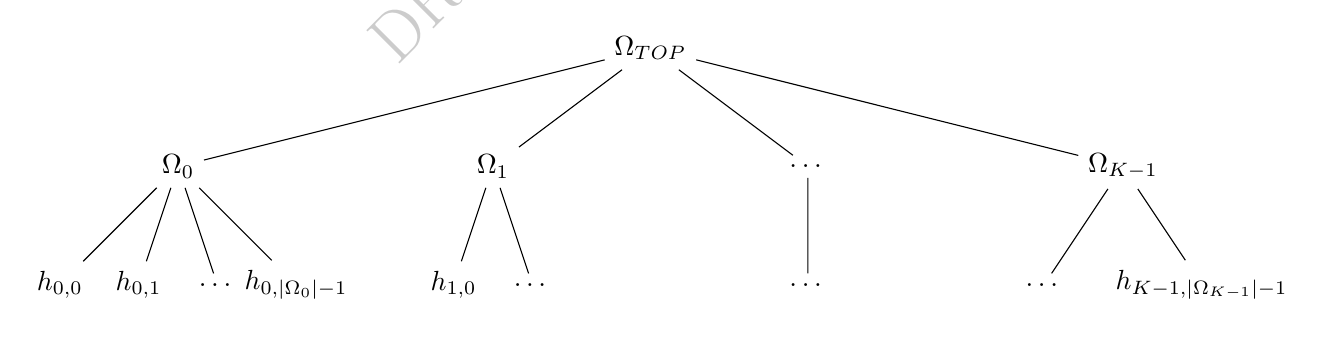
\begin{tikzpicture}
\node {\(\Omega_{TOP}\)} [sibling distance = 4cm]
  child {node {\(\Omega_0\)}  [sibling distance = 1cm]
    child {node {\(h_{0, 0}\)}}
    child {node {\(h_{0, 1}\)}}
    child {node {\dots}}
    child {node {\(h_{0, |\Omega_0| - 1}\)}}
  }
  child {node {\(\Omega_1\)}  [sibling distance = 1cm]
    child {node {\(h_{1, 0}\)}}
    child {node {\dots}}  
  }
  child {node {\dots}
    child {node {\dots}}
  }
  child {node {\(\Omega_{K-1}\)}   [sibling distance = 2cm]
    child {node {\dots}}
    child {node {\(h_{K-1, |\Omega_{K-1}| - 1}\)}}
  };
\end{tikzpicture}

Now we let \(\Omega\) be the set of all outcomes \(\Omega_0 \cup \Omega_1 \cup \dots \Omega_{K-1}\), and we create a relative probability function \(P\) with the following assumptions:

1) If the two outcomes fall under the same component, then their relative probabilities do not change:
\[P(h_{k, i}, h_{k, j}) = P_k(h_{k, i}, h_{k, j})\]

2) If the 2 outcomes fall under different components, then their relative probabilities are given as follows:
\[P(h_{k_1, i}, h_{k_2, j}) = P_k(h_{k_1, i}, \Omega_{k_1}) \cdot  P_{TOP}(\Omega_{k_1}, \Omega_{k_2}) \cdot P_{TOP}(\Omega_{k_2}, h_{k_2, j})\]

Theorem: \(P\) respects the fundamental property

Proof: Fill IN

Theorem: \(P\) is totally comparable if and only if the following three things are true:

1) \(P_{TOP}\) is totally comparable

2) For all \(0 \leq k < K\), \(P_k\) is totally comparable

3) There is at most one component with impossible outcomes with respect to that component. Equivalently, if \(h_{k_1, i}\) and \(h_{k_2, j}\) are two components, and \(P_{k_1}(h_{k_1, i}) = P_{k_2}(h_{k_2, j}) = 0\), then \(k_1 = k_2\). Also equivalently, all components except at most one are totally mutually possible.

Proof: FILL IN



\section{Topology of Relative Probability Spaces}

TODO: Warn people that background in topology is required for this section, and then we can shorten it up!

One of the benefits of relative probability spaces is their properties with respect to limits. Specifically, if we look at the space of (absolute) categorical distributions on \(\Omega\) and we allow the probability of one outcome to approach 1, then all of the other probabilities will be forced down to 0 and become incomparable with one another. In the relative probability space, the information about the ratios of probabilities of the other outcomes can be preserved even as a single outcome reaches a probability of 1.

- What does it mean to take a limit on relative probability space
- What does it mean to approach 1, when if you change 1 value you need to change others as well

Therefore, we want to look at the space of totally comparable relative probability functions. If that space can be shown to be compact, then we know that all limits of such functions are also totally comparable - in other words, the relative probabilites of outcomes and events are preserved even as they both approach zero relative to another event.

The key to defining limits on a space is to first define a topology on that space, which means finding the sets that are open (or intuitively, sets that fully surround all of it's members and don't contain its boundary). This starts with finding a \textit{basis of open sets} from which all other open sets can be constructed through countable unions.

For the absolute probability function, we can use the K-cell, or \(K-1\)-dimentional simplex embedded in \(\mathbb{R}^K\) to get a topology using the standard Euclidean space. For relative probability, we need to build some background mechanisms in order for this to work.

First note that the notion of an open set can change even if a topological space is restricted. For example, on the real number line \(\mathbb{R}\), we take the open interval (0, 1) as an open set (as the term open interval suggests). However, once this is embedded into \(\mathbb{R}^2\), it is now a line segment in a plane and no longer open. It can be thought of as a restriction to an open set on \(\mathbb{R}^2\) to \(\mathbb{R}\). For example, the set \(\{(x, y): x \in (0, 1)\;  \text{and}\;  y \in (-\epsilon, +\epsilon)\}\) given an \(\epsilon > 0\) is such an open set on \(\mathbb{R}^2\). [ILLUSTRATION]

Likewise, an open set on a relative probability space restricted on several outcomes might not be an open set on the relative probability spaces for all of \(\Omega\).

STEP 1: Define the notion of an interior open patch for \(K = 2\)

STEP 2: Using composition, define the notion of an interior open patch for any \(K\).

STEP 3: Define an open patch (not neccesarily interior) using composition. In this case, \(P_{TOP}\) is broken into 2 pieces using a relative probability \(q\) where \(a < q < b\) - but this time it could be \(0 \leq q < b\). The side which could be zero is confined to an open patch, whereas the side that is definitely not zero is further confined to an interior open patch.

Definition: Let an open set on the space of totally mutually possible events on \(\Omega\) correspond to the Euclidean notion of an open set.

Discussion: There's a lot of unpack here, so we'll have to unpack it!

Next: Now we want to space of mutually comparable, but not neccesarily mutually possible.
- Start with a tree interval of mutually possible functions.
- One and only one branch of the tree can have an interval of the form \(\{x: 0 \leq x < a\), where the items below it may well be impossible with respect to items above it.
- That branch could have such a branch below it, etc.
- If you have 2 branches like this that are not ancestors/descendants, then you end up with a tree where 2 branches might be incomparable, which is not allowed.
- If all the brances with 0 included in the interval are descended from each other, then you have an open interval of mutually comparable functions.

Then - use these open intervals to form a basis, and declare that an open set of mutually comparable functions \(P\) is a union of such open intervals.

\subsection{Simple Limit Example}

Let us define a simple relative probability distribution \(P_q\) where \(K = 3\) that is parameterized by the magnitude \(q \in \mathbb{M}\).

Let \(P_q(h_0, h_1) = q\) and \(P_q(h_1, h_2) = 2\).

By the fundamental property, \(P_q(h_0, h_2) :\cong P_q(h_0, h_1) \dot P_q(h_1, h_2) = 2q\).

Now we want to consider the case where the relative probability of \(h_0\) grows infinitely large in comparison to \(h_1\) and \(h_2\).

\[P = lim_{q \rightarrow \infty} P_q\]

We use the following topological definition for the limit in this case: For every open set A of relative probability distributions containing P, there exists an open interval \(B=(b, \infty)\) on \(\mathbb{M}\) such that for every value of \(q \in B\), \(P_q\) is in A.

Proposition: The above limit that defines \(P\) exists, and \(P(h_1, h_2) = 2\). In other words, \(h_2\) is still half as likely as \(h_1\) and that information hasn't been lost on \(P\).

Proof: TODO

\section{Bayesian Inference on Relative Distributions}

A relative probability function represents a belief over the set of potential hypotheses \(\Omega\).

- For each hypothesis, we can also have a likelihood function with data.

- Multiply these two together to get an updated belief function.

- Prove that the updated believe function obeys the fundamental property

Theorem: Once an outcome becomes impossible with respect to another event, it will either remain impossible or become uncomparable.

Theorem: Once two outcome  become uncomparable, they will never be comparable again.

\section{Implementation}

How to implement this in code, and point to open source example.

This can be implemented by storing K values.

For each category, we have a tier. Items in the same tier are comparable. Each Tier has a parent tier, where items in this teir are said to be impossible relative to anything in its ancestor tiers.

For each category, we also store a floating point number called the value, which should be taken as the log of an unnormalized probability. Note that we will not allow inf or NaN here.

Get the relative probability of 2 categories. Algorithm: If they are in the same tier, then subtract their values and take the exp. If they are in different tiers, do a graph search on the tier. If the first is < the second, the answer is 0. If the first is > the second, the answer is 1. And if they are uncomparable, then the answer is Wildcard, NaN.

Generate and indifferent distribution of category K. Algorithm: Create a single tier where all values are set to 0.

Change the relative probability of item \(k_1\) with respect to \(k_2\), and set it to \(q\). Algorithm: UNSURE

Set the probability \(k_1\) to some absolute value with respect to either the whole distribution, or to its tier.

Randomly sample from this distribution. Algorithm: Only look at the top tier.

Randomly sample from this distribution, but remove certain categories. Algorithm: If the top tier categories are gone, look to see if a top tier remains. If there are multiple top tiers, then there's no way to do it!

Ask: Is this distribution totally mutually possible? Algorithm: Look are a single top tier.

Ask: Is it totally mutually comparable? Algorithm: Look for a linear list of tiers.

\section{Future Work}
\subsection{Expansions to infinite spaces}
- Including topological and metric
- Much richer world, more complex mathematics, more applications
- Is it possible to create a univified version of the Hausdorff measure, where objects are categorized by dimention \(d\), and a smaller-dimentional object is always mutually impossible to a larger dimentional object.
\subsection{Connection Surreal Numbers}
- This is greater, richer than the real number system
- Does this abrograte the need for the relative probability function (not for incomparable values)
- If the infinite case is dealt with above, then more questions are raised about both the power of surreal numbers and their suitability
\subsection{Shrinking the Measure Number System}
- We still have a usable system if we want Rational Numbers
- Can this system work for all non-standard probability value systems?
- There is practical application in this work, since computers cannot work with real numbers directly. We implement this system with floating point numbers and this approximation should be good enough for most applications - but can we have a version with more precise arithmetic

\begin{appendices}

\section{Is an Appendix Needed}

\end{appendices}

%\subsubsection*{References}

\begin{thebibliography}{20}

\bibitem{sklar_dirichlet}Sklar, M. (2014). Fast MLE computation for the Dirichlet multinomial. arXiv preprint arXiv:1405.0099.
\bibitem{mendelson}Mendelson, B. (1990). Introduction to topology. Courier Corporation.
\bibitem{bradley}Bradley, T. D., Bryson, T., \& Terilla, J. (2020). Topology: A Categorical Approach. MIT Press.

\end{thebibliography}

This document along with revisions is posted at github as https://github.com/maxsklar/relative-probability-finite-paper. See readme for contact information. Local Maximum Labs is an ongoing effort create an disseminate knowledge on intelligent computing.
\end{document}
